\chapter{Introdução}\label{cap_introducao}

\section{Problemas de Otimização}

Em matemática e ciência da computação, problemas de otimização consistem naqueles em que
a solução é um elemento de um conjunto de candidatos que melhor satisfaz uma determinada
série de condições. Um exemplo clássico dessa classe é o problema da mochila 
(\textit{knapsack problem}, em inglês), no qual
procura-se, dentre um conjunto de itens com diversos preços e pesos, o subconjunto que
maximiza o valor total. Esse valor é calculado somando-se os preços dos itens postos na
mochila. 

Entretanto a solução deve respeitar um vínculo: o peso total dos objetos escolhidos
não deve exceder o peso máximo suportado pela mochila. Ainda que seja possível encontrar a solução exata
desse problema usando algoritmos de programação dinâmica,
a complexidade de tais algoritmos é $ \mathcal{O} (n w) $, onde $n$ é o número de itens e $w$ é a
capacidade da bolsa. Assim, o tempo de execução para muitos itens\trav que é o caso de interesse,
usualmente\trav pode ser mais longo do que o desejado.

Outro exemplo comum de problema de otimização é o de otimização numérica, do qual constituem
solução os pontos de máximo ou mínimo global de uma função 
$ f : \R^n \rightarrow \R $. Tomemos como exemplo simples a função
\begin{equation}
  f(x, y) = \cos(n\pi r)\exp\left(-\frac{r^2}{\sigma^2}\right) \mathcomma
  \label{eq:damped_cos}
\end{equation}
definida no domínio $ [-1, 1] \times [-1, 1] $, cujo gráfico se encontra na Figura \paref{fig:damped_cos}. 
Analiticamente é fácil determinar o ponto de máximo global em $ r = 0 $ usando métodos de cálculo
para funções de múltiplas variáveis. 
Contudo, não é sempre que pode-se dispor de tal facilidade. 
Nos casos em que a função objetivo é de maior complexidade, com domínio contido espaços de maior dimensão; 
em que a função tem evolução temporal; em que a função possui diversas descontinuidades; ou em que a função
depende de variáveis aleatórias, o problema se torna impraticável de resolver de forma analítica. 
Isto posto, como desenvolver um algoritmo para encontrar a solução?

\begin{figure}
  \centering
  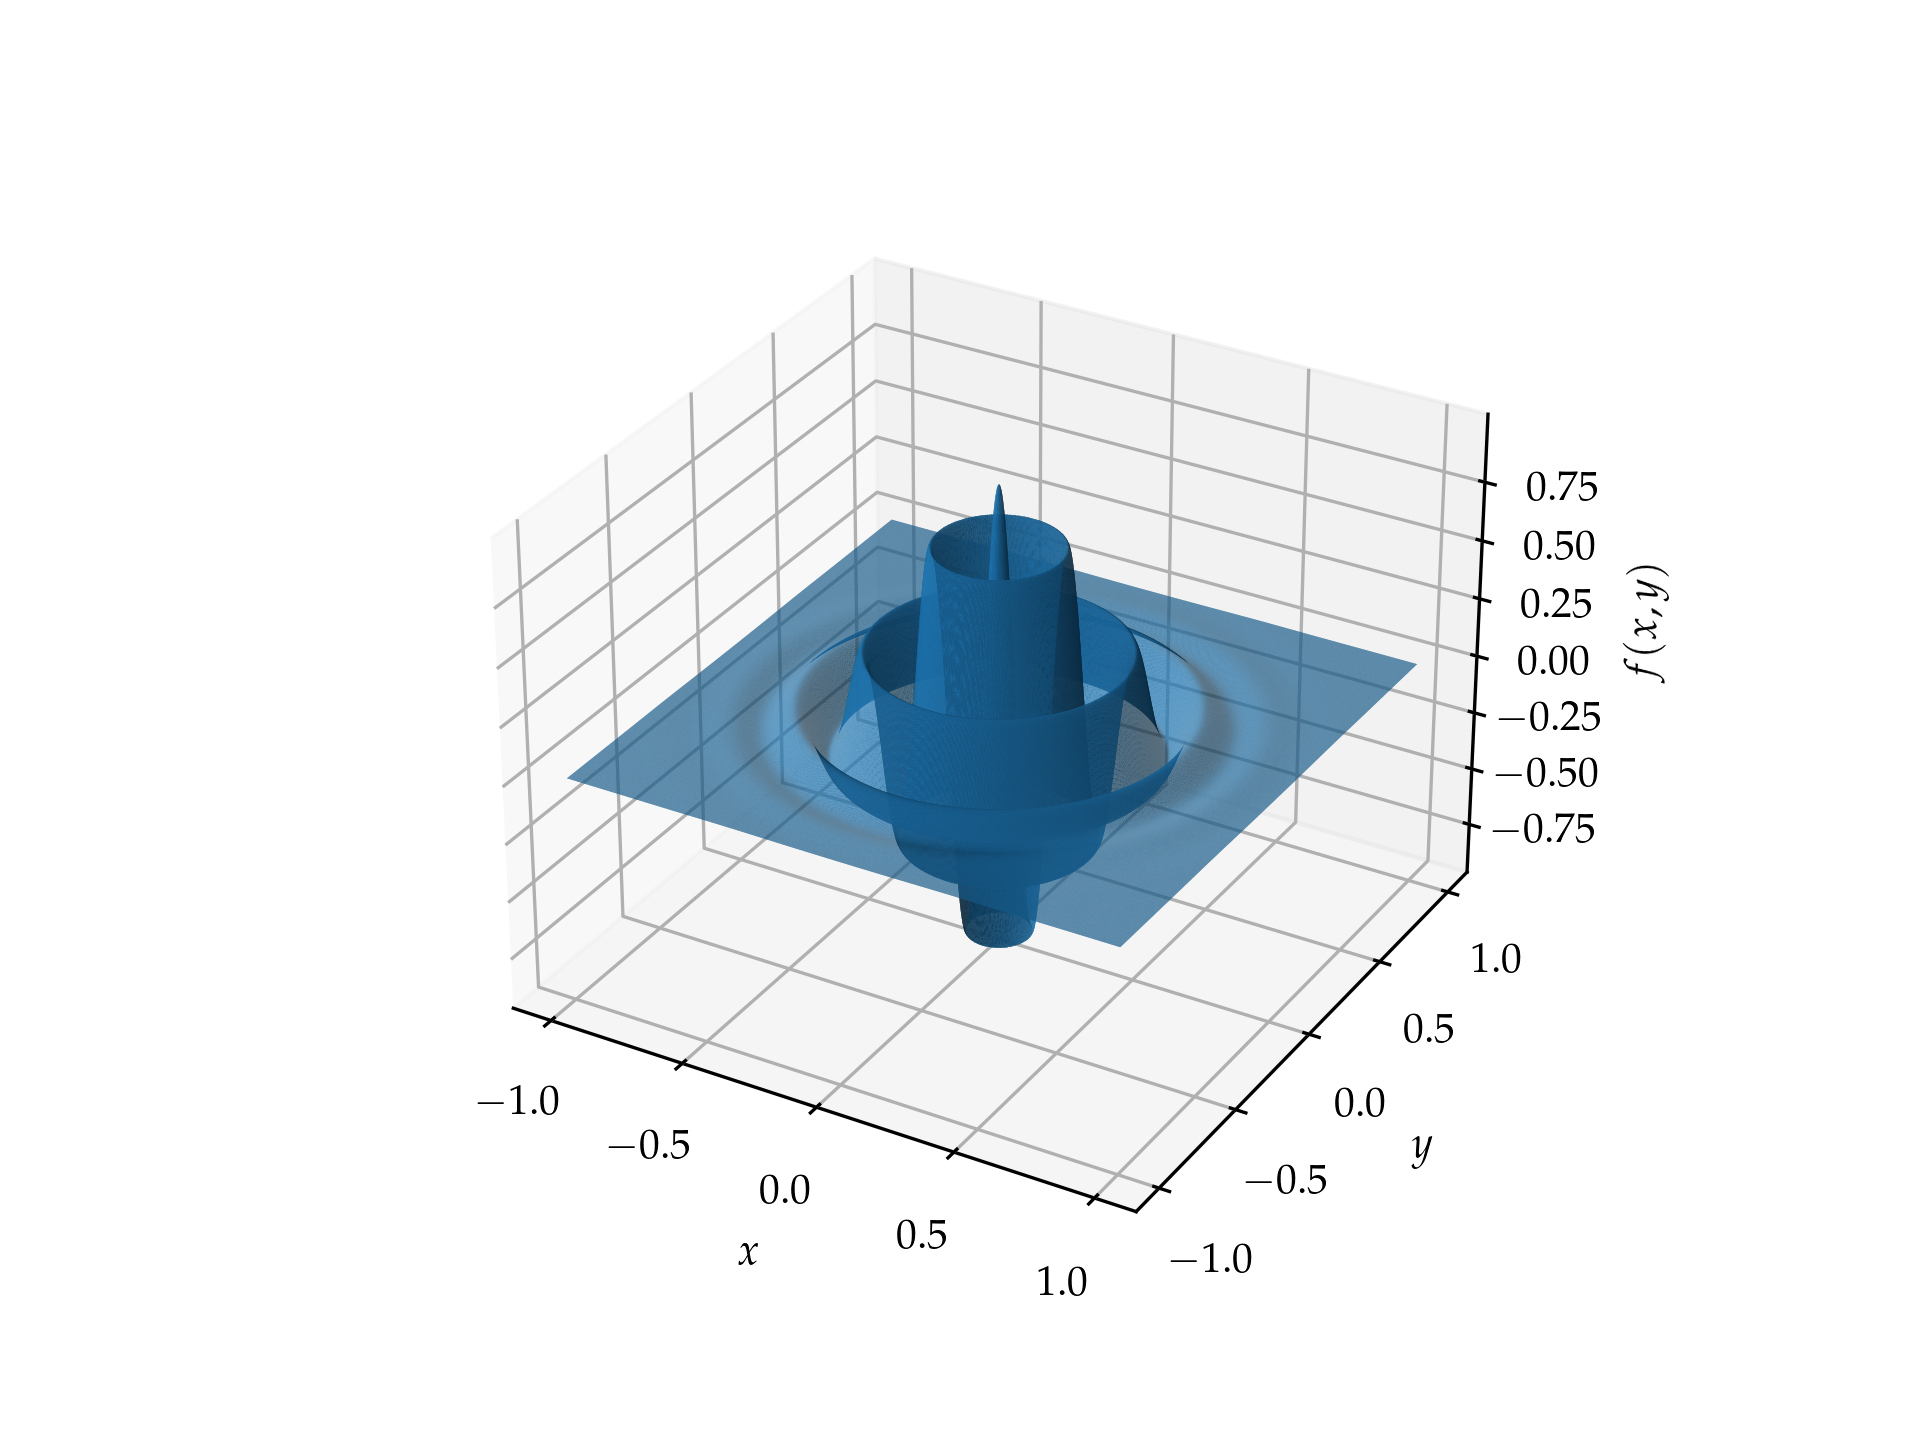
\includegraphics[width=\textwidth]{imagens/damped_cossine.png}
  \caption{Gráfico da função definida na Equação \paref{eq:damped_cos}, com $ n = 9 $ e $ \sigma = 0,4 $.}
  \label{fig:damped_cos}
\end{figure}

Uma classe de algoritmos mais simples que se propõem a resolver esse problema são os algoritmos do
tipo escalada de morro (\textit{hill climbing}, em inglês). 
Sugerido pelo nome, o funcionamento desses algoritmos consiste, resumidamente,
em sortear um ponto inicial no domínio da função, calcular o gradiente da função no ponto, e seguir
na direção resultante por uma distância pré-definida, e repetir esses passos até que o módulo do
vetor gradiente seja próximo de zero, respeitando uma tolerância previamente determinada\cite{goldberg1989ga}. 

O problema com esse tipo de algoritmo é que, quando aplicado em funções como a definida anteriormente, a tendência é
de que a solução encontrada seja um máximo local na grande maioria das vezes. No caso da função definida
pela Equação \paref{eq:damped_cos}, o máximo local só seria encontrado pelo algoritmo se o ponto inicial
fosse tal que $ r < \nicefrac{1}{n} $. Se os pontos iniciais do algoritmo forem gerados aleatoriamente,
para o domínio definido, a probabilidade de um ponto pertencer a esta região é $ P(n) = \nicefrac{\pi}{4n^2} $.
Para $ n = 9 $, como na Figura \paref{fig:damped_cos}, $ P \approx 1\% $. 
Ademais, é possível que esse tipo
de algoritmo indique erroneamente como solução pontos de sela e planícies em determinados casos, o que o
torna ainda menos eficaz para o propósito.

Uma outra categoria de algoritmos que podem resolver ambos os problemas de forma rápida e chegar a uma
solução que se aproxima o suficiente da solução exata são os algoritmos genéticos. Tais algoritmos,
quando bem implementados, podem chegar a uma solução aproximada para o problema da mochila de forma
rápida para valores de $n$ e $w$ ordens de grandeza superiores aos que tornariam praticável o uso da
estratégia proposta anteriormente. 

No problema de otimização numérica, um algoritmo desse tipo é vantajoso pois é capaz de chegar na solução
de forma rápida na maioria dos casos, identificando não só o máximo global, como também os máximos
locais contidos na região de busca. Outra vantagem é que esse método pode ser aplicado sem problemas
em espaços de busca com grande número de dimensões, ou em funções não estacionárias, contínuas ou
descontínuas. Além disso, como será mostrado posteriormente, o algoritmo é paralelizável, o que pode
acelerar a obtenção de uma solução.

\section{O Algoritmo Genético}

Os algoritmos genéticos foram primeiramente desenvolvidos por John H. 
Holland\cite{holland1992ga} na década de 60. Levam esse nome pois sua formulação teve como 
forte influência o processo de evolução natural que fomenta a origem das espécies desde o surgimento da vida
em nosso planeta. Em sua execução, é inicializada uma população de indivíduos da mesma espécie\footnote{
  Isso significa que seus respectivos códigos genéticos possuem a mesma estrutura: mesma número de
  cromossomos com uma mesma quantidade de genes. Assim, pode haver reprodução entre tais indivíduos.
}.
Cada indivíduo corresponde a um candidato a solução do problema de otimização proposto, e tem sua
identidade codificada pelo seu material genético\footnote{
  No caso do problema da mochila, por exemplo, uma
  estrutura natural para o material genético é um cromossomo binário, com $n$ genes, cada um correspondente
  a um objeto do problema. Por outro lado, no problema de otimização numérica, dois cromossomos seriam
  necessários, um para codificar cada coordenada em cada dimensão do espaço de busca.
}.
Então, sob algum critério, é selecionada uma parcela desses indivíduos, a qual dará origem a novos
descendentes, cujos cromossomos serão gerados pela recombinação dos cromossomos correspondentes nos
pais. Nesse passo é introduzida uma probabilidade de mutação nos genes dos filhos. 

Ao final desse processo, descarta-se a parcela não selecionada da população, dando origem a uma nova geração, formada
pelos pais seus filhos. Esse processo é repetido iterativamente até que uma condição de parada seja
atingida. Essa condição pode ser imposta sobre o número de gerações ou sobre o tempo de execução do programa,
por exemplo.
Respeitando as diferenças de implementação em cada passo, devido as peculiaridades de cada tipo de problema
de otimização proposto, essas etapas são presentes em todo algoritmo genético, e são bem resumidas no fluxograma
presente na Figura \paref{fig:ga_flow}.

\begin{figure}
  \centering
  \begin{tikzpicture}
    \node[start_end] (start) {Início};
    \node[io, below=1em of start] (init_pop) {População\\ Inicial};
    \node[process, below=1em of init_pop]  (selection) {Seleção};
    \node[process, below=1em of selection]  (crossover) {Recombinação};
    \node[process, below=1em of crossover]  (mutation) {Mutação};
    \node[decision, below=1em of mutation]  (check) {Condição atingida?};
    \node[document, left=10ex of check] (print_stats) {Informações da\\População};
    \node[start_end, above=10ex of print_stats] (end) {Fim};
    \draw[myarrow=.9] (start.south) --  (init_pop.north);
    \draw[myarrow=.9] (init_pop.south) --  (selection.north);
    \draw[myarrow=.9] (selection.south) --  (crossover.north);
    \draw[myarrow=.9] (crossover.south) --  (mutation.north);
    \draw[myarrow=.9] (mutation.south) -- (check.north);
    \draw[myarrow=.9] (check.east) -- node[description, above] {Não} ([xshift=10ex]check.east) |- (selection.east);
    \draw[myarrow=.9] (check.west) -- node[description, above] {Sim} (print_stats.east);
    \draw[myarrow=.9] (print_stats.north) -- (end.south);
  \end{tikzpicture}
  \caption{Fluxograma geral de um algoritmo genético.}
  \label{fig:ga_flow}
\end{figure}

\section{A Implementação do Algoritmo Genético}

A linguagem de programação escolhida para a implementação do algoritmo foi Python\footnote{
  Versão 3.10.4, com NumPy na versão 1.22.3, e Matplotlib na versão 3.5.1.
  Código disponível em \url{https://github.com/davifeliciano/num_opt_ga}.
}. Amplamente utilizada no meio 
acadêmico, trata-se de uma linguagem de fácil compreensão e aprendizado, além de contar com diversas bibliotecas
já implementadas com o objetivo de resolver problemas recorrentes.

As duas principais bibliotecas utilizadas neste projeto foram NumPy e Matplotlib. 
A primeira se trata de uma biblioteca para manipulação numérica e vetorizada de matrizes. É implementada na linguagem C, 
o que confere performance às operações numéricas, mantendo a facilidade de uso e versatilidade características da linguagem
Python. Já a segunda, se trata de uma biblioteca para a criação de gráficos matemáticos, que será de suma importância
na ilustração de forma clara dos resultados obtidos.

Os detalhes acerca da codificação escolhida para o material genético dos indivíduos, bem como os métodos utilizados
nas etapas de seleção, recombinação e mutação foram propostos em \citeyear{roncaratti2006ga} por \citeauthor{roncaratti2006ga},
e serão abordados de forma breve no capítulo seguinte.
